\chapter{F\'ary--Milnor theorem}

\section{Tame knots}

It is tricky to make a formal definition that captures the intuitive meaning of \emph{knot}.
An attempt to define knots as simple closed curves leads to a pathological examples as the one show on the diagram --- these are so called \emph{wild knots}.
\begin{figure}[h]
\vskip-0mm
\centering
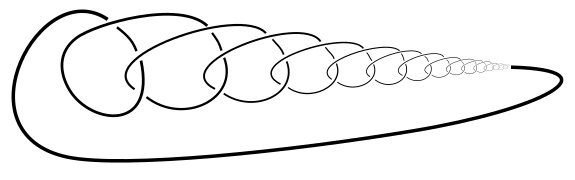
\includegraphics[scale=.6]{pics/Wild_knot}
\vskip0mm
\end{figure}
If one adds that the curve has to be smooth and regular,
then these examples disappear, but it is still a tricky to give right definition of \emph{deformation} --- the following diagram shows 
\begin{figure}[h]
\vskip-0mm
\centering
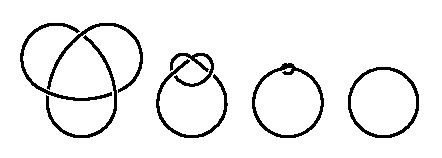
\includegraphics[scale=1]{pics/knot}
\vskip0mm
\end{figure}
that it can not be defined as a continuous family of closed simple smooth regular curves. 
Observe that all curves on the diagram are smooth and regular for all times including the last moment.

We define a \emph{knot} (more precicely \emph{tame knot}) as a simple closed polygonal line in Euclidean space~$\RR^3$.

The notation $\triangle abc$ is used for triangle $abc$; that is a polygonal line with three edges and vertexes $a$, $b$ and $c$.
Let us denote by $\solidtriangle abc$ the convex hull of the points $a$, $b$ and $c$; $\solidtriangle abc$ is the solid triangle with the vertexes $a$, $b$ and $c$.
The points $a$, $b$ and $c$ are assumed to be distinct, but they might lie on one line;
that is, for us a degenerate triangle is a triangle.

We understand a \emph{triangular isotopy} of a knot to be the generation of a new knot from the original one by means of the
following two operations:

Assume $[pq]$ is an edge of the knot and $x$
is a point such that the solid triangle $\solidtriangle pqx$  has no common points with the knot except for the edge $[pq]$.
Then we can replace the edge $[pq]$ in the knot by two adjacent edges $[px]$ and $[xq]$.

We can also perform the inverse operation.
That is, if for two adjacent edges $[px]$ and $[xq]$ of a knot the triangle
$\solidtriangle pqx$ has no common points with the knot except for the points on the edges $[px]$ and $[xq]$,
then we can replace two adjacent edges $[px]$ and $[xq]$ by one edge $[pq]$.

Polygons that arise from one another by a finite sequence of
triangular isotopies are called \emph{isotopic}.

\begin{wrapfigure}{r}{25 mm}
\vskip-0mm
\centering
\includegraphics{mppics/pic-18}
\vskip0mm
\end{wrapfigure}

A knot that is not isotopic to a triangle is called nontrivial.

The trefoil knot shown on the diagram gives a simple example of nontrivial knot.
A proof that the trefoil knot is nontrivial can be found in any textbook on knot theory, we do not give it here.
The most elementary and visual proof is based on the so called \emph{tricolorability} of knot diagrams.   

\begin{thm}{Exercise}\label{ex:triangle-isotopy}
Let $x$ and $y$ be two points on the adjacent edges $[p_1p_2]$ and $[p_2p_3]$ of a knot $\beta=p_1p_2p_3\dots p_n$.
Assume that the solid triangle $\solidtriangle xp_2y$ intersects $\beta$ only along the $[xp_2]\cup [p_2y]$.
Show that the knot $\beta'=p_1xyp_3\dots p_n$ is isotopic to $\beta$.
\end{thm}



\section{F\'ary--Milnor theorem}

We will give few proofs of the following theorem.

\begin{thm}{Theorem}\label{thm:fary-milnor}
The total curvature of any nontrival knot is at least $4\cdot\pi$. 
\end{thm}

The famous F\'ary--Milnor theorem states that the inequality is strict;
that is, the total curvature of any nontrival knot \emph{exceeds} $4\cdot\pi$.
It is easy to construct a trefoil knot with total curvature arbitrary close to $4\cdot\pi$;
therefore this result is optimal.

The question was raised by Karol Borsuk \cite{borsuk} and answered independently by Istv\'an F\'ary and John Milnor \cite{fary, milnor};
latter few other proofs were found.

\section{Milnor's proof}

In the proof we will use the following fact. 

\begin{thm}{Proposition}\label{prop:one-max-one-min}
Assume that a height function $(x,y,z)\to z$ 
has only one local minimum and one local maximum on a closed simple polygonal line and all the vertexes of the polygonal line lie on different height.
Then the line is a trivial knot.
\end{thm}

The proof is a simple application of the definition of isotopy, given in the previous section. 

\begin{wrapfigure}{r}{20 mm}
\vskip-0mm
\centering
\includegraphics{mppics/pic-19}
\vskip0mm
\end{wrapfigure}

\parit{Proof.}
Let $\beta=p_1\dots p_n$ be the closed simple polygonal line
such that the height function $(x,y,z)\to z$ has one local minimum one local maximum.
Note that on each of the two arcs of $\beta$ from min-vertex to max-vertex the height function increases monotonically.

Consider three vertexes with the largest value of the height function;
they have to include the max-vertex and two more.
Note that these three vertexes are consequent in the polygonal line; 
without loss of generality we can assume that they are $p_{n-1},p_n,p_1$.

Note that the solid triangle $\solidtriangle p_{n-1}p_np_1$ does not intersect any edge $\beta$ except the two adjacent edges $[p_{n-1}p_n]\cup[p_np_1]$.
Indeed, if $\solidtriangle p_{n-1}p_np_1$ intersects $[p_1p_2]$,
then, 
since $p_2$ lies below $\solidtriangle p_{n-1}p_np_1$,
$[p_1p_2]$ must intersect $[p_{n-1}p_n]$
which is impossible since $\beta$ is simple.
The same way one can show that $\solidtriangle p_{n-1}p_np_1$ can not intersect $[p_{n-2}p_{n-1}]$.
The remaining edges lie below $\solidtriangle p_{n-1}p_np_1$, hence they can not intersect this triangle.

Applying triangular isotopy, to $\solidtriangle p_{n-1}p_np_1$ we get a closed simple polygonal line $\beta'\z=p_1\dots p_{n-1}$ which is isotopic to $\beta$.

Since all the vertexes $p_i$ have different height,
the assumption of proposition holds for $\beta'$.

Repeating this procedure $n-3$ times we get a triangle.
Hence $\beta$ is a trivial knot.
\qeds

\parit{Milnor's proof of \ref{thm:fary-milnor}.}
Let $\alpha$ be a simple closed polygonal line.
Assume its total curvature is less that $4\cdot\pi$.
Then by Proposition~\ref{prop:tc-crofton}, 
\[\tc\alpha_u<4\cdot\pi\]
for some unit vector $u$.
Moreover, we can assume that $u$ points in a generic direction;
that is, $u$ is not perpendicular to any edge or diagonal of $\alpha$.

The total curvature of $\alpha_u$ is $\pi$ times the number of turns of $\alpha_u$
which has to be an even number.
It follows that number of turns of $\alpha_u$ is at most $2$;
it can not be less than 2 for generic direction and therefore it is $2$.

That is, if we rotate the space so that $u$ pints to the top,
than the height function has exactly one minimum and one maximum;
by Proposition~\ref{prop:one-max-one-min}, $\alpha$ is a trivial knot --- hence the result.
\qeds

\section{F\'ary's proof}

Let us give a sketch of another proof, based on the original idea of Istv\'an F\'ary.

\begin{wrapfigure}{r}{30 mm}
\vskip-0mm
\centering
\includegraphics{mppics/pic-13}
\vskip0mm
\end{wrapfigure}

\parit{F\'ary's proof of \ref{thm:fary-milnor}.}
Consider a projection of the knot to a plane in general position.
That is, we assume that the self-intersections of the projection are at most double and the projection of each edge does not degenerate.
The obtained closed polygonal line $\beta=p_1p_2\dots p_n$ divides the plane into domains, one of which is unbounded, denote it by $U$, and the others are bounded.

First note that all domains can be colored in a chessboard order;
that is, they can be colored in black and white in such a way that domains with common borderline get different colors.
If the unbounded domain gets white color and every other domain is black then one can untie the knot by flipping these domains one by one.

\begin{thm}{Exercise}
Give a formal proof of the last statement; that is, show that if only undbounded domain is white then $\beta$ is isotopic to a triangle. 
\end{thm}

\begin{wrapfigure}{r}{30 mm}
\vskip-4mm
\centering
\includegraphics{mppics/pic-14}
\vskip0mm
\end{wrapfigure}

Therefore among the bounded domains there is a white domain, denote it by $D$.
The domain $D$ can not have a borderline with $U$ since they have the same color.
Fix a point $o$ in this domain.

For each $i$, set 
\begin{align*}
\phi_i&=\pi-\measuredangle p_{i-1}p_ip_{i+1},
\\
\psi_i&=\measuredangle p_{i-1} o p_{i},
\\
\theta_i&=\measuredangle o p_i p_{i+1}.
\end{align*}
Here indexes are taken modulo $n$; in particular, $p_{n}=p_0$.


Note that $\phi_i$ is the external angle at $p_i$;
therefore 
\[\tc\beta= \phi_1+\dots+\phi_n\]

Direct calculations show that 
\[\phi_i\ge \psi_i+\theta_{i-1}-\theta_i.\]
In the two pictures below, $\phi_i$ is the solid angle;
the rest of angles $\psi_i$, $\theta_{i-1}$ and $\theta_i$
are the same.
We have equality on the first picture and strict inequality on the second picture.

\begin{figure}[h]
\vskip-0mm
\centering
\includegraphics{mppics/pic-15}
\vskip0mm
\end{figure}

It follows that 
\[\phi_1+\dots+\phi_n\ge \psi_1+\dots+\psi_n.\]

The last sum 
is the total angle at  which $\beta$ seen from $o$ counted with multiplicity. 
The boundary of $D$ contributes at least $2\cdot\pi$ to this sum and the boundary of $U$ contributes an other $2\cdot\pi$;
since their boundaries do not overlap we get 
\[\psi_1+\dots+\psi_n\ge 4\cdot\pi,\]
hence the result.

This is true for the projection of the knot to any plane in general position.
The remaining planes contribute nothing to the average value.
Therefore by Proposition~\ref{prop:tc-crofton}, the total curvature of the original knot is at least $4\cdot\pi$.
\qeds



\begin{thm}{Exercise}
Construct a closed smooth simple curve with total curvature arbitrary close to $2\cdot\pi$ such that its projection to any plane has at least $10$ self-intersections.   
\end{thm}



\section{Proof of Alexander and Bishop}

Here we sketch a proof of F\'ary--Milnor theorem given by of Stephanie Alexander and Richard Bishop in \cite{alexander-bishop}.

The proof is elementary, but not simple 
(elementary does not mean simple, it means only that it does not use much theory).
It is based on the following two facts that we already familiar with:
\begin{itemize}
\item If a closed polygonal line $\beta'$ is inscribed in a closed polygonal line $\beta$ then 
 \[\tc\beta'\le \tc\beta.\]
\item The total curvature of doubly covered
bigon is $4\cdot\pi$; that is,
\[\tc\beta=4\cdot\pi\]
if $\beta=pqpq$ for two distinct points $p$ and $q$.
Similarly if a quadrilateral is sufficiently close to a doubly covered
bigon, then its total curvature is close to $4\cdot\pi$.
\end{itemize}


\parit{Proof.}
Let $\beta=p_1\dots p_n$ be a closed polygonal line that is not a trivial knot;
that is, one can not get a triangle from $\beta$ by applying a sequence of triangular isotopys defined in the previous section.

We proceed by induction on the number $n \ge 3$.
In the base case $n=3$ the polygonal line $\beta$ is a triangle.
Therefore, by the definition, $\beta$ is a trivial knot --- nothing to prove.

Consider the smallest $n$ for which the statement fail;
that is, there is a closed simple polygonal line $\beta\z=p_1\dots p_n$ that is not a trivial knot such that
\[\tc\beta<4\cdot\pi.
\eqlbl{eq:<4pi}\]
We use the indexes modulo $n$ that is $p_0=p_n$, $p_1=p_{n+1}$ and so on.
Without loss of generality, we may assume that $\beta$ is in general position; 
that is, no four vertexes of $\beta$ lie on one plane. 

Set $\beta_0=\beta$.
If the solid triangle $\solidtriangle p_{0}p_1p_{2}$ intersects $\beta_0$ only by the two adjacent edges,
then applying the corresponding triangular isotopy, we get a knot $\beta'_0$ with $n-1$ edge that is inscribed in $\beta_0$ therefore
\[\tc\beta_0\ge \tc\beta_0'.\]
On the other hand by induction hypothesis 
\[\tc\beta_0'\ge 4\cdot\pi\]
which contradicts \ref{eq:<4pi}.

Choose the first point $w'_1$ on the edge $[p_1p_2]$ so that the line segment $[p_0w'_1]$ 
intersects $\beta_0$.
Denote a point of intersection by $y_1$.

\begin{wrapfigure}{r}{25 mm}
\vskip-0mm
\centering
\includegraphics{mppics/pic-17}
\vskip0mm
\end{wrapfigure}

Choose a point $w_1$ on $[p_1p_2]$ a bit before $w'_1$
(below we explain how close).
Denote by $x_1$ the point on $[p_0w_1]$ that minimize the distance to $y_1$.
This way we get a closed polygonal line 
$\beta_1\z=w_1p_2\dots p_n$ with two marked points $x_1$ and $y_1$.
Denote by $m_1$ the number of edges in the arc $y_1w_1\dots x_1$ of $\beta_1$.

By Exercise~\ref{ex:triangle-isotopy}, $\beta_1$ is isotopic to $\beta_0$;
in particular $\beta_1$ is a nontrivial knot.

Now let us repeat the procedure for the adjacent edges $[w_1b_2]$ and $[b_2b_3]$ of $\beta_1$.
If the solid triangle $\solidtriangle w_1b_2b_3$ intersects $\beta_1$ only at these two adjacent edges, then we get a contradiction with the induction hypothesis the same way as before.
Otherwise we get a new knot $\beta_2=w_1w_2b_3\dots b_n$ with two marked points $x_2$ and $y_2$.
Denote by $m_2$ the number of edges in the broken line $y_2w_3\dots x_2$.

Note that the points $x_1,x_2,y_1,y_2$ can not appear on $\beta_2$ in the same cyclic order;
otherwise the broken line $x_1x_2y_1y_2$ can be made to be arbitrary close to a doubly covered bigon which again contradicts~\ref{eq:<4pi}.%
\footnote{More precisely, the choice of $w_1$ has to be made so that the distance $|x_1-y_1|$ would be much less that all the distances between $y_1$ and any point $z\in\beta\cap \solidtriangle p_1p_2p_3$, so we have
\[\measuredangle y_1zx_1<\tfrac\eps{10},\]
where $\eps=4\cdot\pi-\tc\beta$.
In this case, since $y_2\in \beta\cap \solidtriangle p_1p_2p_3$ and $x_2$ can be taken arbitrary close to $y_2$, we have
\[\tc x_1x_2y_1y_2 > 4\cdot\pi -\eps= \tc\beta\]
which can not happen since $x_1x_2y_1y_2$ is inscribed in $\beta$.}

Therefore we can assume that the arc $x_2w_2\dots y_2$ lies inside of arc $x_1w_1\dots y_1$ in $\beta_2$
and therefore $m_1>m_2$.

Continuing this procedure we get a sequence of polygonal lines $\beta_i\z=w_1\dots w_i p_{i+1}p_n$ with marked points $x_i$ and $y_i$ such that the number of edges $m_i$ from $x_i$ to $y_i$ decreases in $i$.
Clearly $m_i>1$ for any $i$ and $m_1<n$.
Therefore it requires less than $n$ steps we get a contradiction with the induction hypothesis.
\qeds

\begin{wrapfigure}{r}{30 mm}
\vskip-0mm
\centering
\includegraphics{mppics/pic-20}
\vskip0mm
\end{wrapfigure}

\begin{thm}{Exercise}
Suppose that a closed curve $\alpha$ crosses a line at four points $a$, $b$, $c$ and $d$.
Assume that the points $a$, $b$, $c$ and $d$ appear on the line in the same order and they appear on the curve $\alpha$ in the order $a$, $c$, $b$, $d$.
Show that 
\[\tc\alpha\ge 4\cdot\pi.\]
\end{thm}


\begin{thm}{Advanced exercise}
Show that given any real number $\Phi$ there is a knot $\beta$ such that any knot isotopic to $\beta$ has total curvature at least~$\Phi$.   
\end{thm}

\parit{Hint:} Use that there are knots with arbitrary large \emph{bridge number}, see for example \cite{schultens} and the references there in.


